\appendix
\addtocontents{toc}{%
  \protect\vspace{1em}% 
  \protect\noindent \bfseries \appendixtocname\protect\par
  \protect\vspace{-.5em}%
 }
 \renewcommand{\chaptername}{\appendixname}
 
\begin{appendices}

\chapter{Appendix A}

\section{WebRTCService Script} 
\label{app:webrtc_service}

\begin{lstlisting}[caption={WebRTCService.js in application client},label={code:webrtc_service}]
'use strict';

/**
*  services Module
*
* WebRTCService with browser adapter.js function
*/

angular.module('webrtcDemo.services').
	factory('WebRTCService',function () {
		var _ws;//websocket obj
		
		var _RTCPeerConnection;
		var _RTCSessionDescription;
		var _RTCIceCandidate;
		var _getUserMedia;
		var _createIceServer;
		var _attachMediaStream;
		var _reattachMediaStream;
		var _webrtcDetectedBrowser;
		var _webrtcDetectedVersion;

		function _initWebRTC () {
			_RTCPeerConnection = null;
			_RTCSessionDescription = null;
			_RTCIceCandidate = null;
			_getUserMedia = null;
			_createIceServer = null;
			_attachMediaStream = null;
			_reattachMediaStream = null;
			_webrtcDetectedBrowser = null;
			_webrtcDetectedVersion = null;

			_setRTCElement();
		}

		function _setRTCElement() {

			if(navigator.mozGetUserMedia){
				console.log("This appears to be Firefox");

				_webrtcDetectedBrowser = "firefox";
				_webrtcDetectedVersion = parseInt(navigator.userAgent.match(/Firefox\/([0-9]+)\./)[1], 10);

				_RTCPeerConnection = mozRTCPeerConnection;
				_RTCSessionDescription = mozRTCSessionDescription;
  			_RTCIceCandidate = mozRTCIceCandidate;
  			_getUserMedia = navigator.mozGetUserMedia.bind(navigator);

  			// Creates iceServer from the url for FF.
			  _createIceServer = function(url, username, password) {
			    var iceServer = null;
			    var url_parts = url.split(':');
			    if (url_parts[0].indexOf('stun') === 0) {
			      // Create iceServer with stun url.
			      iceServer = { 'url': url };
			    } else if (url_parts[0].indexOf('turn') === 0) {
			      if (_webrtcDetectedVersion < 27) {
			        // Create iceServer with turn url.
			        // Ignore the transport parameter from TURN url for FF version <=27.
			        var turn_url_parts = url.split("?");
			        // Return null for createIceServer if transport=tcp.
			        if (turn_url_parts.length === 1 ||
			            turn_url_parts[1].indexOf('transport=udp') === 0) {
			          iceServer = { 'url': turn_url_parts[0],
			                        'credential': password,
			                        'username': username };
			        }
			      } else {
			        // FF 27 and above supports transport parameters in TURN url,
			        // So passing in the full url to create iceServer.
			        iceServer = { 'url': url,
			                      'credential': password,
			                      'username': username };
			      }
			    }
			    return iceServer;
			  };

  			_attachMediaStream = function(element, stream) {
			    console.log("Attaching media stream");
			    element.mozSrcObject = stream;
			    element.play();
			  };

			  _reattachMediaStream = function(to, from) {
			    console.log("Reattaching media stream");
			    to.mozSrcObject = from.mozSrcObject;
			    to.play();
			  };

			  // Fake get{Video,Audio}Tracks
			  if (!MediaStream.prototype.getVideoTracks) {
			    MediaStream.prototype.getVideoTracks = function() {
			      return [];
			    };
			  }

			  if (!MediaStream.prototype.getAudioTracks) {
			    MediaStream.prototype.getAudioTracks = function() {
			      return [];
			    };
			  }

			}else if(navigator.webkitGetUserMedia){
				console.log("This appears to be Chrome");

				_webrtcDetectedBrowser = "chrome";
				_webrtcDetectedVersion = parseInt(navigator.userAgent.match(/Chrom(e|ium)\/([0-9]+)\./)[2], 10);

			  _RTCPeerConnection = webkitRTCPeerConnection;
			  _RTCSessionDescription = RTCSessionDescription;
			  _RTCIceCandidate = RTCIceCandidate;
			  _getUserMedia = navigator.webkitGetUserMedia.bind(navigator);

			  // Creates iceServer from the url for Chrome.
			  _createIceServer = function(url, username, password) {
			    var iceServer = null;
			    var url_parts = url.split(':');
			    if (url_parts[0].indexOf('stun') === 0) {
			      // Create iceServer with stun url.
			      iceServer = { 'url': url };
			    } else if (url_parts[0].indexOf('turn') === 0) {
			      if (_webrtcDetectedVersion < 28) {
			        // For pre-M28 chrome versions use old TURN format.
			        var url_turn_parts = url.split("turn:");
			        iceServer = { 'url': 'turn:' + username + '@' + url_turn_parts[1],
			                      'credential': password };
			      } else {
			        // For Chrome M28 & above use new TURN format.
			        iceServer = { 'url': url,
			                      'credential': password,
			                      'username': username };
			      }
			    }
			    return iceServer;
			  };

			  // Attach a media stream to an element.
			  _attachMediaStream = function(element, stream) {
			    if (typeof element.srcObject !== 'undefined') {
			      element.srcObject = stream;
			    } else if (typeof element.mozSrcObject !== 'undefined') {
			      element.mozSrcObject = stream;
			    } else if (typeof element.src !== 'undefined') {
			      element.src = URL.createObjectURL(stream);
			    } else {
			      console.log('Error attaching stream to element.');
			    }
			  };

			  _reattachMediaStream = function(to, from) {
			    to.src = from.src;
			  };

			  // The representation of tracks in a stream is changed in M26
			  // Unify them for earlier Chrome versions in the coexisting period
			  if (!webkitMediaStream.prototype.getVideoTracks) {
			    webkitMediaStream.prototype.getVideoTracks = function() {
			      return this.videoTracks;
			    };
			    webkitMediaStream.prototype.getAudioTracks = function() {
			      return this.audioTracks;
			    };
			  }

			  // New syntax of getXXXStreams method in M26
			  if (!webkitRTCPeerConnection.prototype.getLocalStreams) {
			    webkitRTCPeerConnection.prototype.getLocalStreams = function() {
			      return this.localStreams;
			    };
			    webkitRTCPeerConnection.prototype.getRemoteStreams = function() {
			      return this.remoteStreams;
			    };
			  }

			}else{
				console.log("Browser does not appear to be WebRTC-capable");
			}

		}

		return {
			init : function (socket) {
				if(socket){
					//init service with websocket
					_ws = socket;
				}

				_initWebRTC();

			},

			peerConnection : function(config,constraints){
				if(_RTCPeerConnection){
					return new _RTCPeerConnection(config,constraints);
				}
				return null;
			},

			RTCSessionDescription : function(message){
				if(_RTCSessionDescription){
					return new _RTCSessionDescription(message);
				}
				return null;
			},

			RTCIceCandidate : function(options){
				if(_RTCIceCandidate){
						return new _RTCIceCandidate(options);
					}
					return null;
			},

			webrtcDetectedBrowser : function(){
				return _webrtcDetectedBrowser;
			},

			attachMediaStream : function(element, stream){
				return _attachMediaStream(element, stream);
			},

			reattachMediaStream : function(to, from){
				return _reattachMediaStream(to, from);
			},

			getUserMedia : function(constraints, handleUserMedia, handleUserMediaError){
				return _getUserMedia(constraints, handleUserMedia, handleUserMediaError);
			}

		}
	});	
	
\end{lstlisting}

\section{PhoneViewCtrl Script}
\label{app:phone_ctrl}

\begin{lstlisting}[caption={\_setSocketListener() Function in PhoneViewCtrl.js on Application Client},label={code:client_socket}]
function _setSocketListener(socket){

			socket.on('log', function (array){
			  console.log.apply(console, array);
			});

			socket.on('webrtc', function (data){
			  console.log('Received webrtc message:', data);
			  switch(data.type){
			  	case 'register':
				  	if(data.msg == 'success'){
				  		offer2xms = false;
				  		if(data.colleagues.length != 0){
				  			_.map(data.colleagues,function(c){
				  				var contact = _.find($scope.contactsHolder.contacts,function(contact){
				  					return contact.number == c.number;
				  				});
				  				if(contact){
				  					contact.online = true;
				  					$scope.onlines.push(contact);
				  				}
				  			});
				  		}
							_maybeStart();
				  	}
			  		break;
			  	case 'online':
			  		$scope.contactsHolder.contacts = _.map($scope.contactsHolder.contacts,function(c){
			  			if(c.number == data.user.number){
			  				c.online = true;
			  				$scope.onlines.push(c);
			  			}
			  			return c;
			  		})
			  		break;
			  	case 'join conference':

			  		break;
			  	case 'disconnect':
			  		$scope.contactsHolder.contacts = _.map($scope.contactsHolder.contacts,function(c){
			  			if(c.number == data.user.number){
			  				c.online = false;
			  				var i = $scope.onlines.indexOf(c);
					      if(i != -1) {
					        $scope.onlines.splice(i, 1);
					      }
			  				//$scope.onlines.pop(c);
			  			}
			  			return c;
			  		})
			  		break;
			  	case 'offer':
			  		/*
			  		if (!isStarted) {
				      _maybeStart();
				    }
				    pc.setRemoteDescription(WebRTCService.RTCSessionDescription(data));
				    _doAnswer();
				    */
			  		break;
			  	case 'answer':
			  		if(isStarted){
			  			if(data.sdp){
			  				pc.setRemoteDescription(WebRTCService.RTCSessionDescription(data));
			  			}
			  			if(!data.self){
			  				socket.emit('sip',{
						    	type: 'invite',
						    	username: $scope.user.name,
						    	content: {
						    		to: $scope.outPhone.number
						    	}
						    });
			  			}else{
			  				var channel;
			  				if(callDirection === 'outbound'){
			  					channel = 'sip';
			  				}else{
			  					channel = 'webrtc';
			  				}
			  				
			  				socket.emit(channel,{
						    	type: 'answerInvite',
						    	username: $scope.user.name,
						    	conf_id: conf_id
						    });

						    //show answer process notification
								$rootScope.$broadcast('answer-call',{number : $scope.toAnswerPhone.number});

			  			}
					    
			  		}
			  		break;
			  	case 'candidate':
			  		/*
			  		if(isStarted){
			  			var candidate = WebRTCService.RTCIceCandidate({
					    	sdpMLineIndex:data.content.label,
					    	sdpMid:data.content.id,
					      candidate:data.content.candidate
					    });
					    pc.addIceCandidate(candidate);
			  		}
			  		*/
			  		break;
			  	case 'bye':
			  		if(isStarted){
			  			_handleRemoteHangup();
			  		}
			  		break;
			  	case 'createRTCoffer':
						callDirection = data.callDirection;
						conf_id = data.conf_id;
						break;
			  	default:
			  		break;
			  }
			});

			socket.on('sip',function(data){
				console.log('Received sip message:',data);
				switch(data.type){
					case 'createRTCoffer':
						callDirection = data.callDirection;
						break;
					case 'busy':

			  		break;
					default:
						break;
				}
			});
		}

\end{lstlisting}

\section{ChatBoardCtrl Script}
\label{app:chatboard_ctrl}

\begin{lstlisting}[caption={Files Sharing in ChatBoardCtrl.js},label={code:client_fileshare}]
'use strict';


/**
*  Controllers Module
*
* Chat Board Controller
*/
angular.module('webrtcDemo.controllers').
	controller('ChatBoardCtrl',function ($scope,$location,$upload,WebSocketService,storage,appId) {

		$scope.uploadFiles = [];
		$scope.recievedFiles = [];
		$scope.dialog = [];

		var socket;
		var delivery;
		var channelReday = false;

		_initChatBoardView();

		function b64toBlob(b64Data, contentType, sliceSize) {
	    contentType = contentType || '';
	    sliceSize = sliceSize || 512;

	    var byteCharacters = atob(b64Data);
	    var byteArrays = [];

	    for (var offset = 0; offset < byteCharacters.length; offset += sliceSize) {
	        var slice = byteCharacters.slice(offset, offset + sliceSize);

	        var byteNumbers = new Array(slice.length);
	        for (var i = 0; i < slice.length; i++) {
	            byteNumbers[i] = slice.charCodeAt(i);
	        }

	        var byteArray = new Uint8Array(byteNumbers);

	        byteArrays.push(byteArray);
	    }

	    var blob = new Blob(byteArrays, {type: contentType});
	    return blob;
		}

		function _sendMessage(channel,data){
			console.log('Client sending message: ', data);
		  WebSocketService.sendMessage(channel,data);
		}

		function _upload(files){
  		if(channelReday){
  			_.each(files,function(file){

  				var msg = {
  					source: 'Me',
  					number: $scope.user.name,
  					time: moment().calendar(),
  					content: 'Sharing file: ' + file.name,
  					fileAction: false,
						smsAction: false
  				}

  				$scope.dialog.push(msg);

					delivery.send(file);
  			});
  		}
  	}

  	...

		function _initChatBoardView(){
			socket = WebSocketService.getCurrentSocket();

			...

			delivery = new Delivery(socket);

			delivery.on('delivery.connect',function(delivery){
				channelReday = true;
			});

			delivery.on('send.success',function(fileUID){
	  		console.log("file was successfully sent.");
			});

			delivery.on('receive.success',function(file){
	      console.log('receive file');
	      $scope.recievedFiles.push(file);

	      var msg = {
	      	source: 'File Shared',
  				time: moment().calendar(),
  				content: file.name,
  				fileAction: true,
					smsAction: false,
  				file: file.name
	      }

	      $scope.dialog.push(msg);
	    });

			...

		}

		...

		$scope.browserFiles = function(){
			document.getElementById("fileBtn").click();
		}

		$scope.onFileSelect = function($files) {
	    //$files: an array of files selected, each file has name, size, and type.
	    $scope.uploadFiles = $files;
	    _upload($scope.uploadFiles);
  	};

  	$scope.saveFile = function(msg,filename){
  		var tempFile = _.find($scope.recievedFiles,function(file){
				return file.name == filename;
			});

  		var fileBlob = b64toBlob(tempFile.data,tempFile.mimeType);
  		saveAs(fileBlob, tempFile.name);

  		var i = $scope.recievedFiles.indexOf(tempFile);
      if(i != -1) {
        $scope.recievedFiles.splice(i, 1);
      }
  		//$scope.recievedFiles.pop(tempFile);
  		msg.fileAction = false;
			msg.smsAction = false;
  	}

  	$scope.deleteFile = function(msg,filename){
  		var tempFile = _.find($scope.recievedFiles,function(file){
				return file.name == filename;
			});

  		var i = $scope.recievedFiles.indexOf(tempFile);
      if(i != -1) {
        $scope.recievedFiles.splice(i, 1);
      }
  		//$scope.recievedFiles.pop(tempFile);
  		msg.fileAction = false;
			msg.smsAction = false;
  	}
  	...
  		});
\end{lstlisting}


\chapter{Appendix B}

\section{Socket.IO Implementation Script} 
\label{server:socket}

\begin{lstlisting}[caption={socket.js on Application Server},label={code:server_socket}]
SocketManager.prototype.listen = function(server){
  var self = this;
  clients = {};
  sipClients = {};
  callRequests = {};
  conversations = {};

  io = socketio.listen(server);

  io.sockets.on('connection', _handlerSocket);

  _handlerSip();
}

function _handlerSocket(socket) {
  var delivery = dl.listen(socket);

  // convenience function to log server messages on the client
  function log(){
    var array = [">>>"];
    for (var i = 0; i < arguments.length; i++) {
      array.push(arguments[i]);
    }
      socket.emit('log', array);
  }

  socket.on('sip',function (data){
    log('Got sip message:', data);

    switch(data.type){
      case 'register':
        if(data.username != ""){
          gw.register(data.content.browserClient,function(result){
            socket.emit('sip',result);
          });
        }
        break;
      case 'invite':
        var callerClient = clients[data.username];
        var calleeClient = clients[data.content.to];

        if(!callerClient.inConference){
          xmsManager.createConference({
            type: "audiovideo",
            max_p: 9,
            reserve: 0,
            layout: 0,
            caption: "yes"
          },function(conf_id){
            callerClient.conf_id = conf_id;
            conversations[conf_id] = _createConversation(conf_id);

            xmsManager.joinConference(callerClient.local_identifier,conf_id,{
              caption: "webrtc: " + data.username,
              region: 0,
              audio: "sendrecv",
              video: "sendrecv"
            },function(connected){
              console.log(data.username + ' joined conference : ' + connected);
              callerClient.inConference = true;
              conversations[conf_id].inboundContacts.push(data.username);
              socket.join(conf_id.toString());
            });

            if(calleeClient){
              callerClient.socket.emit('webrtc',{
                type: "ringing",
                number: calleeClient.number
              });

              calleeClient.callreq_id = callerClient.callreq_id;
              callRequests[callerClient.callreq_id].callee = calleeClient;

              calleeClient.socket.emit('webrtc',{
                type: "createRTCoffer",
                inComingNumber: data.username,
                callDirection: 'inbound',
                conf_id: conf_id
              });
            }else{
              _inviteOutboundCall(data.username,data.content.to);
            }   
            
          });

        }else{
          if(calleeClient){
            callerClient.socket.emit('webrtc',{
              type: "ringing",
              number: calleeClient.number
            });

            calleeClient.callreq_id = callerClient.callreq_id;
            callRequests[callerClient.callreq_id].callee = calleeClient;

            calleeClient.socket.emit('webrtc',{
              type: "createRTCoffer",
              inComingNumber: data.username,
              callDirection: 'inbound',
              conf_id: callerClient.conf_id
            });
          }else{
            _inviteOutboundCall(data.username,data.content.to);
          }
          
        }
        break;
      case 'answerInvite':
        var client = clients[data.username];
        var req = callRequests[client.callreq_id];

        if(!client.inConference){
          xmsManager.createConference({
            type: "audiovideo",
            max_p: 9,
            reserve: 0,
            layout: 0,
            caption: "yes"
          },function(conf_id){
            client.conf_id = conf_id;
            conversations[conf_id] = _createConversation(conf_id);

            xmsManager.joinConference(client.local_identifier,conf_id,{
              caption: "webrtc: " + data.username,
              region: 0,
              audio: "sendrecv",
              video: "sendrecv"
            },function(connected){
              console.log(data.username + ' joined conference : ' + connected);
              client.inConference = true;
              conversations[conf_id].inboundContacts.push(data.username);
              socket.join(conf_id.toString());
            });
            
            xmsManager.joinConference(req.caller.remote_identifier,conf_id,{
              caption: "sip: " + unq(req.caller.number),
              region: 0,
              audio: "sendrecv",
              video: "inactive"
            },function(connected){
              console.log(req.caller.number + ' joined conference : ' + connected);
              req.caller.conf_id = conf_id;
              conversations[conf_id].outboundContacts.push(req.caller.number);
              callRequests[client.callreq_id].end = true;
            });

          });
        }else{

          xmsManager.joinConference(req.caller.remote_identifier,client.conf_id,{
            caption: "sip: " + unq(req.caller.number),
            region: 0,
            audio: "sendrecv",
            video: "inactive"
          },function(connected){
            console.log(req.caller.number + ' joined conference : ' + connected);
            req.caller.conf_id = client.conf_id;
            conversations[client.conf_id].outboundContacts.push(req.caller.number);
            callRequests[client.callreq_id].end = true;
          });

        }
        break;
      default:
        break;
    }
  });

  socket.on('webrtc', function (data) {
    log('Got webrtc message:', data);
    
    switch(data.type){
      case 'answerInvite':
        var client = clients[data.username];

        xmsManager.joinConference(client.local_identifier,data.conf_id,{
          caption: "webrtc: " + data.username,
          region: 0,
          audio: "sendrecv",
          video: "sendrecv"
        },function(connected){
          console.log(data.username + ' joined conference : ' + connected);
          client.inConference = true;
          client.conf_id = data.conf_id;
          conversations[data.conf_id].inboundContacts.push(data.username);
          socket.join(data.conf_id.toString());
          socket.broadcast.to(data.conf_id.toString()).emit('webrtc',{
            type: 'join conference',
            colleague: client.username,
            conf_id: data.conf_id
          });
          callRequests[client.callreq_id].end = true;
        });
        break;
      case 'answer':
      /*
        clients[data.username].role = 'callee';
        var call = clients[data.username];
        
        if(call.endIceCandidate){
          xmsManager.updateLocalSDP(data.content.sdp,call,function(){
            
            xmsManager.joinXMSCall(call,function(rs){
              console.log("join call response: \n" + rs);

              gw.sendAnswer(data.username,
                call.sipInviteRequest,
                call.remote_xmsSDP,
                function(){
                  console.log('200 ok answer sent');
                });

            });
          });
        }
      */
        break;
      case 'offer':
        var client = clients[data.username];

        if(!data.content.self){
          var id = uuid.v1();
          client.callreq_id = id;

          callRequests[id] = _createCallRequest(id);
          callRequests[id].caller = client;
          
        }else{

          /*
          gw.sendAnswer(data.username,
            clients[data.username].sipInviteRequest,
            clients[data.username].remote_xmsSDP,
            function(){
              console.log('200 ok answer sent');
          });
          */
        }
        
        if(client.inConference){
          socket.emit('webrtc',{
            type: "answer",
            self: data.content.self
          });
        }
        
        break;
      case 'register':
        clients[data.username] = {};
        _resetClient(data.username,data.host,socket,delivery);

        socket.join(data.host);

        var colleagues = _und.map(clients,function(client,key){
          if(client.host == data.host && key != data.username){
            return {
              name: client.username,
              number: client.number,
              online: true
            };
          }
        });

        colleagues = _und.filter(colleagues,function(client){
          return client != null;
        });

        socket.emit('webrtc',{
          type: 'register',
          msg: 'success',
          colleagues: colleagues
        });
        
        socket.broadcast.to(data.host).emit('webrtc', {
          type: 'online',
          user: {
            name: data.username,
            number: clients[data.username].number,
            online: true
          }
        });

        break;
      case 'endCandidate':
        var client = clients[data.username];
        client.endIceCandidate = true;
        
        var role = callRequests[client.callreq_id].caller.number == data.username ? 'caller' : 'callee';

        console.log('webrtc:endCandidate: ' + role + ' sdp: ' + data.content.sdp);

        if(client.local_xmsSDP == '' || client.local_identifier == ''){
            xmsManager.createXMSCall({
            callType: 'webrtc',
            sdp: data.content.sdp
          },function(xmsSdp,id){
            client.local_xmsSDP = xmsSdp;
            client.local_identifier = id;

            socket.emit('webrtc',{
              type: "answer",
              sdp: xmsSdp,
              self: data.content.self
            });
          });
        }else{
          xmsManager.updateLocalSDP(data.content.sdp,client,function(sdp){
            client.local_xmsSDP = sdp;
            socket.emit('webrtc',{
              type: "answer",
              sdp: sdp,
              self: data.content.self
            });
          });
        }

        break;
      case 'candidate':
        
        break;
      case 'hangup':
        
        try{
          var client = clients[data.username];
          var numberClient = clients[data.pairNumber] ? clients[data.pairNumber] : sipClients[data.pairNumber];

          if(!numberClient){

            gw.sendCancel(data.username,data.pairNumber,function(){
              console.log(data.username + 'cancel the call');

              callRequests[client.call_req].end = true;

            });

            var conf = conversations[client.conf_id];

            if(!client.inConference || conf.inboundContacts + conf.outboundContacts <= 1){

              xmsManager.deleteXMSCall(client.local_identifier,function(rs){
                if(rs.statusCode === 204){
                  console.log('hangup: ' + client.username);
                  client.socket.emit('webrtc',{ type: 'bye'});
                  
                  _resetClient(client.username,client.host,client.socket,client.delivery);
                  
                }
              });

            }

          }else{

            if(numberClient.type === 'webrtc' && data.status === 'on'){
              var conf = conversations[client.conf_id];
              var i = conf.inboundContacts.indexOf(client.username);
              if(i != -1) {
                conf.inboundContacts.splice(i, 1);
              }
              //conf.inboundContacts.pop(client.username);

              xmsManager.deleteXMSCall(client.local_identifier,function(rs){
                if(rs.statusCode === 204){
                  console.log('hangup: ' + client.username);
                  client.socket.emit('webrtc',{ type: 'bye'});

                  try{
                    if(conf.inboundContacts.length + conf.outboundContacts.length > 1){
                      socket.broadcast.to(client.conf_id).emit('webrtc',{
                        type: 'forward',
                        number: client.number,
                        newNumber: conf.outboundContacts.length != 0 ? conf.outboundContacts[0] : conf.inboundContacts[0],
                        webrtcOnly: conf.outboundContacts.length == 0 ? true : false
                      });
                    }
                  }catch(e){
                    console.log('RUNTIME ERROR:webrtc:hangup:forward: ', e);
                  }
                  
                  _resetClient(client.username,client.host,client.socket,client.delivery);
                  
                }
              });

              if(conf.outboundContacts.length == 0 && conf.inboundContacts.length == 1){
                xmsManager.deleteXMSCall(numberClient.local_identifier,function(rs){
                  if(rs.statusCode === 204){
                    console.log('hangup to delete: ' + numberClient.username);
                    numberClient.socket.emit('webrtc',{ 
                      type: 'bye',
                      number: client.number
                    });
                    _resetClient(numberClient.username,numberClient.host,numberClient.socket,numberClient.delivery);
                    var i = conf.inboundContacts.indexOf(numberClient.username);
                    if(i != -1) {
                      conf.inboundContacts.splice(i, 1);
                    }
                    //conf.inboundContacts.pop(numberClient.username);
                    xmsManager.deleteXMSConference(conf.id,function(rs){
                      if(rs.statusCode === 204){
                        console.log('webrtc:hangup:conference resource: ' + conf.id + ' delete success.');
                        delete conf;
                      }
                    });
                  }
                });
              }else if(conf.outboundContacts.length == 1 && conf.inboundContacts.length == 0){
                var sipNo = conf.outboundContacts[0];
                var sipClient = sipClients[sipNo];

                xmsManager.deleteXMSCall(sipClient.remote_identifier,function(rs){
                  if(rs.statusCode === 204){
                    var i = conf.outboundContacts.indexOf(sipClient.number);
                    if(i != -1) {
                      conf.outboundContacts.splice(i, 1);
                    }
                    //conf.outboundContacts.pop(sipClient.number);

                    var call_req = _und.find(callRequests,function(q){//TODO: first one match bug
                      if(q.caller.type == 'webrtc'){
                        return q.callee.number == sipClient.number;
                      }else{
                        return q.caller.number == sipClient.number;
                      }
                    });

                    var pair = call_req.caller.type == 'webrtc' ? call_req.caller : call_req.callee;

                    gw.sendBye(pair.username,function(){
                      console.log('bye to number: ' + sipClient.number);
                    });

                    xmsManager.deleteXMSConference(conf.id,function(rs){
                      if(rs.statusCode === 204){
                        console.log('webrtc:hangup:conference resource: ' + conf.id + ' delete success.');
                        delete conf;
                      }
                    });
                  }
                });
              }

            }else if(numberClient.type === 'webrtc' && data.status === 'off'){
              console.log('busy: ' + client.username);

              var conf = conversations[numberClient.conf_id];

              numberClient.socket.emit('webrtc',{ 
                type: 'busy',
                source: client.username
              });

              if(conf.outboundContacts.length == 0 && conf.inboundContacts.length == 1){
                xmsManager.deleteXMSCall(numberClient.local_identifier,function(rs){
                  if(rs.statusCode === 204){
                    console.log('busy to delete: ' + numberClient.username);
                    numberClient.socket.emit('webrtc',{ type: 'bye'});
                    _resetClient(numberClient.username,numberClient.host,numberClient.socket,numberClient.delivery);
                    var i = conf.inboundContacts.indexOf(numberClient.username);
                    if(i != -1) {
                      conf.inboundContacts.splice(i, 1);
                    }
                    //conf.inboundContacts.pop(numberClient.username);

                    xmsManager.deleteXMSConference(conf.id,function(rs){
                      if(rs.statusCode === 204){
                        console.log('webrtc:hangup:conference resource: ' + conf.id + ' delete success.');
                        delete conf;
                      }
                    });
                  }
                });
              }

            }else if(numberClient.type === 'sip' && data.status === 'on'){
              var conf = conversations[client.conf_id];
              var i = conf.inboundContacts.indexOf(client.username);
              if(i != -1) {
                conf.inboundContacts.splice(i, 1);
              }
              //conf.inboundContacts.pop(client.username);

              xmsManager.deleteXMSCall(client.local_identifier,function(rs){
                if(rs.statusCode === 204){
                  console.log('hangup: ' + client.username);
                  client.socket.emit('webrtc',{ type: 'bye'});

                  if(conf.inboundContacts.length + conf.outboundContacts.length > 1){
                    socket.broadcast.to(client.conf_id).emit('webrtc',{
                      type: 'forward',
                      number: client.number,
                      newNumber: conf.outboundContacts.length != 0 ? conf.outboundContacts[0] : conf.inboundContacts[0],
                      webrtcOnly: conf.outboundContacts.length == 0 ? true : false
                    });
                  }

                  if(conf.inboundContacts.length == 0){
                    xmsManager.deleteXMSCall(numberClient.remote_identifier,function(rs){
                      if(rs.statusCode === 204){
                        var i = conf.outboundContacts.indexOf(numberClient.number);
                        if(i != -1) {
                          conf.outboundContacts.splice(i, 1);
                        }
                        //conf.outboundContacts.pop(numberClient.number);

                        var call_req = _und.find(callRequests,function(q){//TODO: first one match bug
                          if(q.caller.type == 'webrtc'){
                            return q.callee.number == numberClient.number;
                          }else{
                            return q.caller.number == numberClient.number;
                          }
                        });

                        var pair = call_req.caller.type == 'webrtc' ? call_req.caller : call_req.callee;

                        gw.sendBye(pair.username,function(){
                          console.log('bye to number: ' + numberClient.number);
                        });

                        xmsManager.deleteXMSConference(conf.id,function(rs){
                          if(rs.statusCode === 204){
                            console.log('sip:hangup:conference resource: ' + conf.id + ' delete success.');
                            delete conf;
                          }
                        });

                      }
                      
                    });
                  }

                  _resetClient(client.username,client.host,client.socket,client.delivery);

                }
              });

            }else if(numberClient.type === 'sip' && data.status === 'off'){

              gw.sendBye(client.username,function(){
                console.log('bye to number: ' + numberClient.number);
              });

            }

          }

        }catch(e){
          console.log('RUNTIME ERROR:sip:hangup: ', e);
        }

        break;
      default:
        
        break;
    }
  });

  socket.on('message',function(data){

    log('Got text message:', data);

    var client = clients[data.source];

    try{

      if(client.conf_id && data.type === 'IM'){
        socket.broadcast.to(client.conf_id.toString()).emit('message',data);

        var conference = conversations[client.conf_id];
        if(conference.outboundContacts.length != 0){
          _und.each(conference.outboundContacts,function(sipNumber,key){
            data.toNumber = sipNumber;
            _sendSMS(data,function(result){
              client.socket.emit('message',{
                type: 'IM Report',
                status: result,
                content: data.content,
                toNumber: sipNumber
              });
            });
          });
        }

      }else if(data.type === 'SMS'){
        _sendSMS(data,function(result){
          client.socket.emit('message',{
            type: 'SMS Report',
            status: result,
            content: data.content,
            toNumber: data.toNumber,
            comment: data.comment
          });
        });
      }

    }catch(e){
      console.log('RUNTIME ERROR:message: ', e);
    }

  });

  socket.on('disconnect', function() {

    var lostClient = _und.find(clients,function(client,key){
      return client.socket.id == socket.id;
    });

    if(lostClient){

      var conf = lostClient.conf_id ? conversations[lostClient.conf_id] : undefined;
      if(conf){
        var i = conf.inboundContacts.indexOf(lostClient.username);
        if(i != -1) {
          conf.inboundContacts.splice(i, 1);
        }
        //conf.inboundContacts.pop(lostClient.username);
      }

      if(lostClient.local_identifier){
        xmsManager.deleteXMSCall(lostClient.local_identifier,function(rs){
          if(rs.statusCode === 204){
            console.log('disconnect: ' + lostClient.username);
          }
        });
      }

      delete clients[lostClient.username];

      socket.broadcast.to(lostClient.host).emit('webrtc',{
        type: 'disconnect',
        user: {
          name: lostClient.username,
          number: lostClient.number,
          online: false
        }
      });

      gw.unregister(lostClient.username);
    }

  });

  delivery.on('receive.success',function(file){

    var sendingClient = _und.find(clients,function(client,key){
      return client.socket.id == socket.id;
    });

    fs.writeFile(file.name,file.buffer, function(err){
      if(err){
        console.log('File could not be saved.');
      }else{
        console.log('File saved.');
        _und.each(clients,function(client,key){
          //if(client.conf_id == sendingClient.conf_id && client.username != sendingClient.username){
          if(sendingClient.conf_id && client.conf_id == sendingClient.conf_id && client.username != sendingClient.username){

            client.socket.emit('message',{
              content: 'Sharing file: ' + file.name + ' ...',
              source: sendingClient.username,
              number: sendingClient.number,
              action: false
            });

            client.delivery.send({
              name: file.name,
              path : './' + file.name
            });

          }
        });

        fs.unlink('./' + file.name);
      };
    });
  });

}
\end{lstlisting}

\section{SIP Implementation Script} 
\label{server:sip}

\begin{lstlisting}[caption={sip.js on Application Server},label={code:sipjs}]
function SipGateway(config){
	EventEmitter.call(this);
	this.config = config || {
		realm: os.hostname(),
		hostPublicAddress: 'xxx.xxx.xxx.xxx',
		hostPort: 5060,
		hostBranch: 'z9hG4bK-' + uuid.v1()
	};
	this.init();
}

util.inherits(SipGateway, EventEmitter);

function rstring() {
	return Math.floor(Math.random() * 1e6).toString();
}

function unq(a) {
  if(a && a[0] === '"' && a[a.length-1] === '"')
    return a.substr(1, a.length - 2);
  return a;
}

function createRegister(user){
	return {
	  method: 'REGISTER',
	  uri: 'sip:' + user.hostname,
	  headers: 
	  {
	  	'call-id': user.callid,
	  	cseq: {method: 'REGISTER', seq: ++user.seq},
	  	from: {name: '', uri: 'sip:' + user.name + '@' + user.hostname, params: { tag: user.tag }},
	    to: {name: '', uri: 'sip:' + user.name + '@' + user.hostname},
	    expires: 3600,
	  	contact:  [{
      	uri: 'sip:' + user.name + '@'+ hostPublicAddress + ':' + hostPort
      }]

	  }
	}
}

function createInvite(client, to){
  return {
		method: 'INVITE',
		uri: 'sip:' + to + '@'+  client.hostname,
		headers: {
			'call-id': client.callid,
			cseq: {
				method: 'INVITE',
				seq: 1
			},
			from: {
        name: '',
				uri: 'sip:' + client.name + '@'+ client.hostname,
				params: {
					tag: client.tag
				}
			},
			to: {
				uri: 'sip:' + to +'@'+ client.hostname
			},
			expires: 3600,
			contact: [{name: '',
				uri: 'sip:' + client.name + '@'+ hostPublicAddress + ':' + hostPort
			}]
		}
  }
}

function createInviteACK(rs,client,sdp){
	var uri = rs.headers.contact[0].uri.split(';');
	if(uri[0].split(':').length != 3){
		uri[0] = uri[0] + ':5060';
	}
	return {
		method: 'ACK',
		uri: uri[0],
		headers: {
			'call-id': rs.headers['call-id'],
			cseq: {
				method: 'ACK',
				seq: rs.headers.cseq.seq
			},
			from: rs.headers.from,
			to: rs.headers.to,
			authorization: client.inviteAuth,
			'content-type': 'application/sdp'
		},
		content: sdp
	}
}

function createAnswerOK(rq,client,sdp){
	var rs = sip.makeResponse(rq, 200, 'OK');
	
	rs.headers.to.params.tag = client.tag;

	rs.headers.contact = [{
  	uri: 'sip:' + client.name + '@'+ hostPublicAddress + ':' + hostPort
  }];

  rs.headers.expires = 3600;
	rs.headers['content-type'] = 'application/sdp';
	//rs.headers['Allow'] = 'INVITE, ACK, CANCEL, BYE, NOTIFY, REFER, MESSAGE, OPTIONS, INFO, SUBSCRIBE';
	//rs.headers['Supported'] = 'replaces';
	rs.content = sdp;

	return rs;
}

function createBye(client){
	var to,from;

	if(client.name != sip.parseUri(client.from.uri).user){
		from = client.to;
		to = client.from;
	}else{
		from = client.from;
		to = client.to;
	}

	return {
	  method: 'BYE',
	  uri: 'sip:' + client.hostname + ':5060',
	  headers: 
	  {
	  	'call-id': client.callid,
	  	cseq: {method: 'BYE', seq: 3},
	  	from: from,
	    to: to,
	  	contact:  [{
      	uri: 'sip:' + client.name + '@'+ hostPublicAddress + ':' + hostPort
      }],
      authorization: client.authorization

	  }
	}
}

function createCancel (client,to) {

	//util.debug("createCancel: \n" + util.inspect(client, false, null));

	return {
	  method: 'CANCEL',
	  uri: 'sip:' + to + '@' + client.hostname,
	  headers: 
	  {
	  	'call-id': client.callid,
	  	cseq: {method: 'CANCEL', seq: 2},
			from: {
        name: '',
				uri: 'sip:' + client.name + '@'+ client.hostname,
				params: {
					tag: client.tag
				}
			},
			to: {
				uri: 'sip:' + to +'@'+ client.hostname
			},
      authorization: client.inviteAuth

	  }
	}
}

function createSMS(client,to,msg){

	return {
		method: 'MESSAGE',
		uri: 'sip:' + to + '@'+  client.hostname,
		headers: {
			'call-id': client.callid,
			cseq: {
				method: 'MESSAGE',
				seq: 1
			},
			from: {
        name: '',
				uri: 'sip:' + client.name + '@'+ client.hostname,
				params: {
					tag: client.tag
				}
			},
			to: {
				uri: 'sip:' + to +'@'+ client.hostname
			},
			authorization: client.authorization,
			'content-type': 'text/plain',
			'content-length': msg.length
		},
		content: msg
	}

}

SipGateway.prototype.init = function () {
	var self = this;
	realm = this.config.realm;
	hostPublicAddress = this.config.hostPublicAddress;
	hostPort = this.config.hostPort;
	hostBranch = this.config.hostBranch;
	registry = {};

	sip.start({
		port: hostPort,
	  logger: { 
	    send: function(message, address) { util.debug("send\n" + util.inspect(message, false, null)); },
	    recv: function(message, address) { util.debug("recv\n" + util.inspect(message, false, null)); }
	  },
	  publicAddress: hostPublicAddress,
	  tcp: false
	},
	function(rq) {
		
	  try {
	    if(rq.method === 'REGISTER') {  
	      util.debug('request register');
	      //looking up user info
	      var username = sip.parseUri(rq.headers.to.uri).user;
	      
	      registry[username] = rq.headers.contact;
	      
	      //var rs = sip.makeResponse(rq, 200, 'Ok');
	      //rs.headers.contact = rq.headers.contact;
	      //sip.send(rs);
	    }
	    else if(rq.method === 'INVITE') {

	      var username = sip.parseUri(rq.uri).user;
	      var contact = registry[username];
	      
	      var rs = sip.makeResponse(rq, 100, 'Trying');
	      sip.send(rs);

	      if(contact) {
	      	registry[username].callid = rq.headers['call-id'];
	      	registry[username].tag = rstring();
	      	registry[username].from = rq.headers.from;
					registry[username].to = rq.headers.to;

	        self.emit('SIPREMOTE',{
	        	type: 'INVITE',
	        	content:{
	        		fromNumber: sip.parseUri(rq.headers.from.uri).user,
	        		toNumber: username,
	        		inviteRequest: rq
	        	}
	        });
	        
	        rs = sip.makeResponse(rq, 180, 'Ringing');
					sip.send(rs);
	      }
	      else {
	        sip.send(sip.makeResponse(rq, 404, 'Not Found'));
	      }

	    }
	    else if(rq.method === 'BYE'){
	    	var endNumber = sip.parseUri(rq.headers.to.uri).user;
	    	var sipNumber = sip.parseUri(rq.headers.from.uri).user;
	    	//console.log(endNumber);
	    	var rs = sip.makeResponse(rq, 200, 'Ok');
	    	sip.send(rs);
	    	self.emit('SIPREMOTE', {
	    		type: 'BYE',
	    		content:{
	    			endNumber: endNumber,
	    			sipNumber: sipNumber
	    		}
	    	});
	    }
	    else if(rq.method === 'ACK'){
	    	util.debug("sip ACK: \n" + util.inspect(rq, false, null));
				
				var username = sip.parseUri(rq.uri).user;
	    	registry[username].answerAcked = true;
	    }
	    else if(rq.method === 'CANCEL'){
	    	var endNumber = sip.parseUri(rq.headers.to.uri).user;
	    	var sipNumber = sip.parseUri(rq.headers.from.uri).user;
	    	//console.log(endNumber);
	    	var rs = sip.makeResponse(rq, 200, 'Ok');
	    	sip.send(rs);
	    	self.emit('SIPREMOTE', {
	    		type: 'CANCEL',
	    		content:{
	    			endNumber: endNumber,
	    			sipNumber: sipNumber
	    		}
	    	});
	    }
	    else {
	      sip.send(sip.makeResponse(rq, 405, 'Method Not Allowed'));
	    }
	  } catch(e) {
	    util.debug(e);
	    util.debug(e.stack);

	    sip.send(sip.makeResponse(rq, 500, "Server Internal Error"));
	  }
	  
	});

	
}

function _register(client,callback){

	var rq = createRegister(client);

	sip.send(rq,function(rs){

		if(rs.status === 401){
			var user = client;
			var creds = { user: user.name, password: user.password, realm: user.hostname };

			rq.headers['cseq'].seq++;
	    rq.headers.via.shift();
	    rq.headers['call-id'] = user.callid;
	    client.seq = rq.headers['cseq'].seq;

	    digest.signRequest(creds, rq, rs, creds);
			sip.send(rq,function(rs){
				if(rs.status === 200){
					
					client.authorization = rq.headers.authorization;

					if(!client.registerTimer){
						client.registerTimer = setInterval(function(){
							console.log('register timer');
							_register(client);
						},parseInt(rs.headers.expires)*1000);
					}

					if(callback){
						callback({type: 'register',msg: 'success'});
					}
				}else{
					if(callback){
						callback({type: 'register',msg: 'failed'});
					}
				}
			});
		}else if(rs.status === 200){
			if(callback){
				callback({type: 'register',msg: 'success'});
			}
		}
		
	});

}


SipGateway.prototype.register = function(client,callback){
	registry[client.name] = {
		name : client.name,
		password : client.pwd,
		hostname : client.host,
		callid : rstring() + '@' + hostPublicAddress,
		tag: rstring(),
		registerTimer: null,
		seq: 0
	};

	_register(registry[client.name],callback);
}

SipGateway.prototype.unregister = function(username){

	clearInterval(registry[username].registerTimer);
	
}

SipGateway.prototype.invite = function(from,to,callback){
	var self = this;
	registry[from].callid = rstring() + '@' + hostPublicAddress;
	registry[from].tag = rstring();

	var client = registry[from];

	var invite_rq = createInvite(client,to);

	client.answerAcked = false;

	sip.send(invite_rq,function(rs){
		if(rs.status === 100){
			client.answerAcked = false;
		}else if(rs.status === 180){
			client.answerAcked = false;
		}
		else if(rs.status === 401){
			//util.debug("invite response: \n" + util.inspect(rs, false, null));

			//util.debug("invite before digest: \n" + util.inspect(invite_rq, false, null));

			invite_rq.headers['cseq'].seq++;
	    invite_rq.headers.via.shift();
	    invite_rq.headers['call-id'] = client.callid;

	    var creds = { user: client.name, password: client.password, realm: unq(rs.headers['www-authenticate'][0].realm) };

			var new_invite_req = digest.signRequest(creds, invite_rq, rs, creds);
			registry[from].inviteAuth = new_invite_req.headers.authorization;
			registry[from].invite_req = new_invite_req;
			//util.debug("invite to be sent: \n" + util.inspect(invite_rq, false, null));

			sip.send(new_invite_req,function(rs){

				if(rs.status === 200){
					//util.debug("second invite response: \n" + util.inspect(rs, false, null));
					if(!client.answerAcked){
						client.answerAcked = true;
						callback(rs);
					}
				}else if(rs.status === 100){

					self.emit('SIPREMOTE', {
		    		type: 'TRYING',
		    		content:{
		    			clientNumber: from,
		    			sipNumber: to
	    			}
		    	});

				}else if(rs.status === 180){

					self.emit('SIPREMOTE', {
		    		type: 'RINGING',
		    		content:{
		    			clientNumber: from,
		    			sipNumber: to
	    			}
		    	});

				}else if(rs.status === 486){

					self.emit('SIPREMOTE', {
		    		type: 'BUSY',
		    		content:{
		    			clientNumber: from,
		    			sipNumber: to
	    			}
		    	});

				}
			});
		}else if(rs.status === 200)
			if(!client.answerAcked){
				client.answerAcked = true;
				callback(rs);
			}
	});
}

SipGateway.prototype.ackInvite = function(from,rs,xmsSDP,callback){
	var client = registry[from];
	var ack = createInviteACK(rs,client,xmsSDP);
	
	util.debug("ack message: \n" + util.inspect(ack, false, null));

	client.from = ack.headers.from;
	client.to = ack.headers.to;

	sip.send(ack);

	callback();//not really callback since there is no response for ack message from server

}

SipGateway.prototype.sendTrying = function(rq){
	var rs = sip.makeResponse(rq, 100, 'Trying');
	sip.send(rs);
}

SipGateway.prototype.sendRing = function(to,rq){
	var client = registry[to];

	var rs = sip.makeResponse(rq, 180, 'Ringing');
	
	rs.headers.to.params.tag = registry[to].tag;

	sip.send(rs);
}

SipGateway.prototype.sendAnswer = function(to,rq,xmsSDP,callback){
	var client = registry[to];
	registry[to].answerAcked = false;

	//var rs = sip.makeResponse(rq, 100, 'Trying');
	//sip.send(rs);

	//rs = sip.makeResponse(rq, 180, 'Ringing');
	//sip.send(rs);

	var ok = createAnswerOK(rq,client,xmsSDP);

	sip.send(ok);

	callback();

}

SipGateway.prototype.sendBye = function(number,callback){
	var client = registry[number];

	var bye = createBye(client);

	sip.send(bye,function(rs){
		if(rs.status === 200){
			callback();
		}
	});
}

SipGateway.prototype.sendCancel = function(from,to,callback){
	var client = registry[from];

	var cancel = createCancel(client,to);

	util.debug("sip:Cancel: \n" + util.inspect(cancel, false, null));

	sip.send(cancel,function(rs){
		if(rs.status === 200){
			callback();
		}
	});
}

SipGateway.prototype.sendBusy = function(rq,callback){

	var busy = sip.makeResponse(rq, 486, 'Busy');
	
	sip.send(busy,function(rs){
		if(rs.status === 200){
			callback();
		}
	});
}

SipGateway.prototype.sendSMS = function(from,to,msg,callback){

	var client = registry[from];

	var sms = createSMS(client,to,msg);

	sip.send(sms,function(rs){
		if(rs.status === 200){
			callback();
		}
	});

}

module.exports.SipGateway = SipGateway;
\end{lstlisting}


\section{XMS Implementation Script} 
\label{server:xms}

\begin{lstlisting}[caption={xms.js on Application Server},label={code:xms}]
XmsManager.prototype.createXMSCall = function(data,callback){
  var requestContent = "<web_service version=\"1.0\">";
  requestContent += "\n<call";
  requestContent += " sdp=\"" + data.sdp.replace(/\r\n/g, "&#xA;") + "\"";
  if(data.callType === 'webrtc'){
    requestContent += " encryption=\"dtls\"" + " ice=\"yes\"";
  }
  requestContent += " media=\"audiovideo\"" + " signaling= \"no\"/>";
  requestContent += "\n</web_service>";

  console.log(requestContent);
  var req = http.request({
    host: xmsAddress,
    port: xmsPort,
    method: 'POST',
    path: xmsPath + 'calls?appid=' + xmsAppId,
    headers: {
      'Accept' : 'application/xml',
      'Content-Type' : 'application/xml',
      'Content-Length' : requestContent.length
    }
  }, function(res) {
    var resData = '';
    console.log('createXMSCall:STATUS: ' + res.statusCode);
    console.log('createXMSCall:HEADERS: ' + JSON.stringify(res.headers));
    res.setEncoding('utf8');
    
    res.on('data', function (chunk) {
      resData += chunk;
    }).on('end', function() {
      if(resData != ''){
        xmlparser.parseString(resData,function(err,result){
          var xmsSdp = result['web_service']['call_response'][0]['$'].sdp;
          var id = result['web_service']['call_response'][0]['$'].identifier;

          var regex = new RegExp(xmsAddress,"g");
          pub_xmsSdp = xmsSdp.replace(regex,xmsPublicAddress);
          console.log('after create call sdp: ' + pub_xmsSdp);

          callback(pub_xmsSdp.replace(/\n/g,"\r\n"),id);
        });
      }
    });
  });

  req.write(requestContent);
  req.end();
}

XmsManager.prototype.joinXMSCall = function(call,callback){
  var requestContent = "<web_service version=\"1.0\">";
  requestContent += "\n<call>";
  requestContent += "\n<call_action>";
  requestContent += "\n<join call_id=\"" + call.remote_identifier + "\"/>";
  requestContent += "\n</call_action>";
  requestContent += "\n</call>";
  requestContent += "\n</web_service>";

  var joinPath = xmsPath + 'calls/' + call.local_identifier + '?appid=' + xmsAppId;

  var req = http.request({
    host: xmsAddress,
    port: xmsPort,
    method: 'PUT',
    path: joinPath,
    headers: {
      'Accept' : 'application/xml',
      'Content-Type' : 'application/xml',
      'Content-Length' : requestContent.length
    }
  }, function(res) {
    var resData = '';
    console.log('joinXMSCall:STATUS: ' + res.statusCode);
    console.log('joinXMSCall:HEADERS: ' + JSON.stringify(res.headers));
    res.setEncoding('utf8');
    
    res.on('data', function (chunk) {
      resData += chunk;
    }).on('end', function() {
      if(resData != ''){
        callback(resData);
      }
    });
  });

  req.write(requestContent);
  req.end();  
}

XmsManager.prototype.updateLocalSDP = function(newSDP,call,callback){
  var requestContent = "<web_service version=\"1.0\">";
  requestContent += "\n<call" + " sdp=\"" 
    + newSDP.replace(/\r\n/g, "&#xA;") + "\"";
  requestContent += " encryption=\"dtls\"" + " ice=\"yes\"";
  requestContent += " media=\"audiovideo\"" + " signaling= \"no\"/>";
  requestContent += "\n</web_service>";

  var updatePath = xmsPath + 'calls/' + call.local_identifier + '?appid=' + xmsAppId;
  //console.log('update request content: '+ requestContent);

  var req = http.request({
    host: xmsAddress,
    port: xmsPort,
    method: 'PUT',
    path: updatePath,
    headers: {
      'Accept' : 'application/xml',
      'Content-Type' : 'application/xml',
      'Content-Length' : requestContent.length
    }
  }, function(res) {
    var resData = '';
    console.log('updateLocalSDP:STATUS: ' + res.statusCode);
    console.log('updateLocalSDP:HEADERS: ' + JSON.stringify(res.headers));
    res.setEncoding('utf8');
    
    res.on('data', function (chunk) {
      resData += chunk;
    }).on('end', function() {
      if(resData != ''){
        xmlparser.parseString(resData,function(err,result){
          var xmsSdp = result['web_service']['call_response'][0]['$'].sdp;
          
          //console.log('after update sdp: ' + xmsSdp);
          if(xmsSdp){
            xmsSdp = xmsSdp.replace(xmsAddress,xmsPublicAddress);
            callback(xmsSdp.replace(/\n/g,"\r\n"));
          }else{
            callback(null);
          }
          
        });
      }
    });
  });

  req.write(requestContent);
  req.end();    
}

XmsManager.prototype.createConference = function(options,callback){
  var requestContent = "<web_service version=\"1.0\">"; 
  requestContent += "\n<conference type=\"" + options.type + "\" max_parties=\"" + options.max_p + "\" reserve=\"" + options.reserve + "\"";
  requestContent += " layout=\"" + options.layout + "\" caption=\"" + options.caption + "\"";
  requestContent += " caption_duration=\"30s\" beep=\"yes\" clamp_dtmf=\"yes\" auto_gain_control=\"yes\" echo_cancellation=\"yes\" />";
  requestContent += "\n</web_service>" 

  //console.log("createConference: " + requestContent);
  var createConfPath = xmsPath + '/conferences?appid=' + xmsAppId;
  //console.log("createConference path: " + createConfPath);
  
  var req = http.request({
    host: xmsAddress,
    port: xmsPort,
    method: 'POST',
    path: createConfPath,
    headers: {
      'Accept' : 'application/xml',
      'Content-Type' : 'application/xml',
      'Content-Length' : requestContent.length
    }
  }, function(res) {
    var resData = '';
    console.log('createConference:STATUS: ' + res.statusCode);
    console.log('createConference:HEADERS: ' + JSON.stringify(res.headers));
    res.setEncoding('utf8');
    
    res.on('data', function (chunk) {
      resData += chunk;
    }).on('end', function() {
      if(resData != ''){
        xmlparser.parseString(resData,function(err,result){
          var conf_id = result['web_service']['conference_response'][0]['$'].identifier;
          
          callback(conf_id);
          
        });
      }
    });
  });

  req.write(requestContent);
  req.end();
}

XmsManager.prototype.joinConference = function(call_id,conf_id,options,callback){
  var requestContent = "<web_service version=\"1.0\">";
  requestContent += "\n<call>";
  requestContent += "\n<call_action>";
  requestContent += "\n<add_party conf_id=\"" + conf_id + "\" caption=\"" + options.caption + "\"";
  requestContent += " region=\"" + options.region + "\" audio=\"" + options.audio + "\" video=\"" + options.video + "\" />";
  requestContent += "\n</call_action>";
  requestContent += "\n</call>";
  requestContent += "\n</web_service>";

  console.log("joinConference: " + requestContent);
  var joinPath = xmsPath + 'calls/' + call_id + '?appid=' + xmsAppId;

  var req = http.request({
    host: xmsAddress,
    port: xmsPort,
    method: 'PUT',
    path: joinPath,
    headers: {
      'Accept' : 'application/xml',
      'Content-Type' : 'application/xml',
      'Content-Length' : requestContent.length
    }
  }, function(res) {
    var resData = '';
    console.log('joinConference:STATUS: ' + res.statusCode);
    console.log('joinConference:HEADERS: ' + JSON.stringify(res.headers));
    res.setEncoding('utf8');
    
    res.on('data', function (chunk) {
      resData += chunk;
    }).on('end', function() {
      if(resData != '' && res.statusCode === 200){
          
        callback('yes');
          
      }
    });
  });

  req.write(requestContent);
  req.end();
}

XmsManager.prototype.deleteXMSCall = function(callId,callback){
  var deletePath = xmsPath + 'calls/' + callId + '?appid=' + xmsAppId;

  var req = http.request({
    host: xmsAddress,
    port: xmsPort,
    method: 'DELETE',
    path: deletePath
  },function(res){
    console.log('deleteXMSCall:STATUS: ' + res.statusCode);
    console.log('deleteXMSCall:HEADERS: ' + JSON.stringify(res.headers));
    res.setEncoding('utf8');

    callback(res);
  });

  req.end();
}

XmsManager.prototype.deleteXMSConference = function(confId,callback){

  var deletePath = xmsPath + 'conferences/' + confId + '?appid=' + xmsAppId;

  var req = http.request({
    host: xmsAddress,
    port: xmsPort,
    method: 'DELETE',
    path: deletePath
  },function(res){
    console.log('deleteXMSConference:STATUS: ' + res.statusCode);
    console.log('deleteXMSConference:HEADERS: ' + JSON.stringify(res.headers));
    res.setEncoding('utf8');

    callback(res);
  });

  req.end();

}

module.exports.XmsManager = XmsManager;
\end{lstlisting}

\section{MSG Implementation Script} 
\label{server:msg}

\begin{lstlisting}[caption={msg.js on Application Server},label={code:msg}]
MsgManager.prototype.login = function(loginDto,success,fail){
	
	var loginStr = JSON.stringify(loginDto);

	var options = {
		host: msgRestUrl,
		path: '/your/url/here/loginWithDto',
		method : 'POST',
		headers: {
			"Accept" : "application/json",
			"Content-Type" : "application/json",
			'Content-Length' : loginStr.length
		}
	};

	var req = https.request(options, function(res) {
		var resData = '';
	  console.log("MSG:LOGIN:statusCode: ", res.statusCode);
	  console.log("MSG:LOGIN:headers: ", res.headers);
	  res.setEncoding('utf8');

	  res.on('data', function (chunk) {
      resData += chunk;
    }).on('end', function() {
    	if(resData != ''){
    		var jsonObject = JSON.parse(resData);
    		if(jsonObject.code === 200){
    			success(jsonObject,res.headers['set-cookie'][0]);
    		}else{
    			fail(jsonObject);
    		}
    	}
    });
	});

	req.write(loginStr);
	req.end();

	req.on('error', function(e) {
	  console.error(e);
	  fail(e);
	});

}

MsgManager.prototype.sendSMS = function(organization,login,cookie,msgObj,success,fail){

	var msgStr = JSON.stringify(msgObj);
	console.log(msgObj);

	var options = {
		host: msgRestUrl,
		path: '/your/url/here/sms',
		method : 'POST',
		headers : {
			"Accept" : "application/json",
			"Content-Type" : "application/json",
			"organization" : organization,
			"login" : login,
			"Cookie" : cookie,
			'Content-Length' : msgStr.length
		}
	};

	var req = https.request(options, function(res) {
		var resData = '';
	  console.log("MSG:SENDSMS:statusCode: ", res.statusCode);
	  console.log("MSG:SENDSMS:headers: ", res.headers);
	  res.setEncoding('utf8');

	  res.on('data', function (chunk) {
      resData += chunk;
    }).on('end', function() {
    	if(resData != ''){
    		var jsonObject = JSON.parse(resData);
    		console.log('MSG:SENDSMS:jsonObject:',jsonObject);
    		if(jsonObject.code === 200){//TODO: check report values as true
    			success();
    		}else{
    			fail();
    		}
    	}
    });
	});

	req.write(msgStr);
	req.end();

	req.on('error', function(e) {
	  console.error(e);
	  fail();
	});

}

module.exports.MsgManager = MsgManager;
\end{lstlisting}

\chapter{Appendix C}

\section{WebRTC in Dart} 
\label{research:dart_webrtcctrl}

\begin{lstlisting}[caption={WebRTCCtrl in Dart application client},label={code:dart_webrtcctrl}]
library webRTCCtrl;

import 'package:angular/angular.dart';
import 'dart:html';
import 'package:webrtcDemo/speaker/speack_client.dart';

@NgController(
  selector : '[webrtc-ctrl]',
  publishAs : 'ctrl'
)

class WebRTCCtrl {

  static const String SERVER_URL = "ws://127.0.0.1:3001";

  String websocketUrl = SERVER_URL;

  WebRTCCtrl() {
    _initConnection();
  }

  void _initConnection(){
    var speaker = new SpeakerClient(websocketUrl, room: 'room');

    speaker.createStream(audio: true, video: true ).then((stream) {
      var video = new VideoElement()
        ..autoplay = true
        ..src = Url.createObjectUrl(stream);

      document.body.append(video);
    });

    speaker.onAdd.listen((message) {
      var video = new VideoElement()
        ..id = 'remote${message['id']}'
        ..autoplay = true
        ..src = Url.createObjectUrl(message['stream']);

      document.body.append(video);
    });

    speaker.onLeave.listen((message) {
      document.query('#remote${message['id']}').remove();
    });
  }
}
\end{lstlisting}

\chapter{Appendix D}

\section{AngularJs Files Structure} 
\label{code:angularjs_structure}

\begin{figure}
	\centering
    	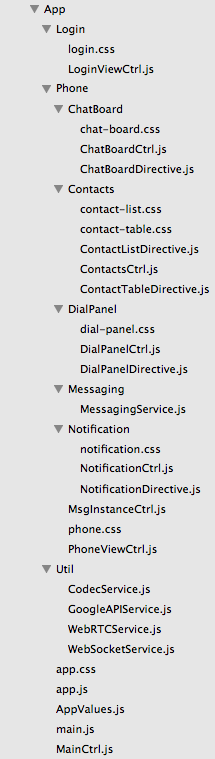
\includegraphics[height=0.45\textheight,natwidth=610,natheight=642]{figs/angularjs_structure.png}
  	\caption{Prototype Application AngularJs Files}
  	\label{fig:angularjs_structure}
\end{figure}

\end{appendices}